\pgfplotsset{width=.98\linewidth, height=5cm}
\begin{figure}[h]
	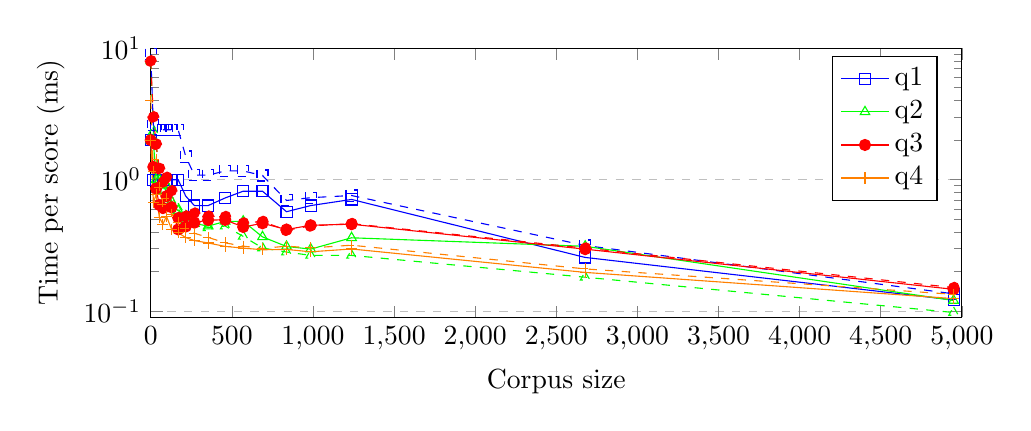
\begin{tikzpicture}[scale=1]
	\begin{axis}[
	xlabel={Corpus size},
	ylabel={Time per score (ms)},
	xmin=0, xmax=5000,
	ymin=0.09, ymax=10,
	legend pos=north east,
	ymajorgrids=true,
	grid style=dashed,
	ymode=log,
	%xmode=log,
	]
	
	    \addplot[
        color=blue,
        mark=square,
        samples=100
        ]
        coordinates {
(0,2)
(16,1)
(33,1)
(53,1)
(75,1)
(97,1)
(128,1)
(169,1)
(216,0.75)
(269,0.636363636363636)
(354,0.636363636363636)
(459,0.727272727272727)
(570,0.818181818181818)
(689,0.818181818181818)
(837,0.571428571428571)
(986,0.636363636363636)
(1238,0.708333333333333)
(2678,0.256756756756757)
(4949,0.121951219512195)
 };

    \addplot[
color=blue,
dashed,
mark=square,
samples=100
]
coordinates {
	(0,9)
	(16,2.6)
	(33,2.4)
	(53,2.4)
	(75,2.4)
	(97,2.4)
	(128,2.4)
	(169,2.4)
	(216,1.5)
	(269,1.08333333333333)
	(354,1.08333333333333)
	(459,1.16666666666667)
	(570,1.16666666666667)
	(689,1.07692307692308)
	(837,0.695652173913043)
	(986,0.730769230769231)
	(1238,0.758620689655172)
	(2678,0.316455696202532)
	(4949,0.135802469135802)
};

	\addplot[
        color=green,
        mark=triangle,
        ]
        coordinates {
(0,2)
(16,2)
(33,1)
(53,1)
(75,0.636363636363636)
(97,0.909090909090909)
(128,0.631578947368421)
(169,0.583333333333333)
(216,0.529411764705882)
(269,0.465116279069767)
(354,0.444444444444444)
(459,0.482142857142857)
(570,0.483333333333333)
(689,0.367816091954023)
(837,0.311111111111111)
(986,0.296969696969697)
(1238,0.362068965517241)
(2678,0.311926605504587)
(4949,0.120833333333333)
        };

\addplot[
color=green,
dashed,
mark=triangle,
]
coordinates {
	(0,8)
	(16,2.33333333333333)
	(33,1.88888888888889)
	(53,1)
	(75,0.823529411764706)
	(97,0.914285714285714)
	(128,0.686274509803922)
	(169,0.602941176470588)
	(216,0.489130434782609)
	(269,0.471698113207547)
	(354,0.431818181818182)
	(459,0.444444444444444)
	(570,0.370967741935484)
	(689,0.302788844621514)
	(837,0.282131661442006)
	(986,0.266149870801034)
	(1238,0.265957446808511)
	(2678,0.181582360570687)
	(4949,0.09796573875803)
};

	\addplot[
        color=red,
        mark=*,
        ]
        coordinates {
(0,2)
(16,1.25)
(33,0.857142857142857)
(53,0.642857142857143)
(75,0.608695652173913)
(97,0.75)
(128,0.617647058823529)
(169,0.419354838709677)
(216,0.441176470588235)
(269,0.471428571428571)
(354,0.49438202247191)
(459,0.495049504950495)
(570,0.4375)
(689,0.466666666666667)
(837,0.418478260869565)
(986,0.450777202072539)
(1238,0.459090909090909)
(2678,0.296703296703297)
(4949,0.146924829157175)
        };

\addplot[
color=red,
dashed,
mark=*,
]
coordinates {
	(0,8)
	(16,3)
	(33,1.85714285714286)
	(53,1.21428571428571)
	(75,0.956521739130435)
	(97,1.04166666666667)
	(128,0.823529411764706)
	(169,0.516129032258065)
	(216,0.529411764705882)
	(269,0.557142857142857)
	(354,0.528089887640449)
	(459,0.524752475247525)
	(570,0.46875)
	(689,0.481481481481481)
	(837,0.41304347826087)
	(986,0.44559585492228)
	(1238,0.463636363636364)
	(2678,0.302197802197802)
	(4949,0.151480637813212)
};

	\addplot[
        color=orange,
        mark=+,
        ]
        coordinates {
(0,2)
(16,0.666666666666667)
(33,0.769230769230769)
(53,0.517241379310345)
(75,0.46)
(97,0.528301886792453)
(128,0.421686746987952)
(169,0.394736842105263)
(216,0.363636363636364)
(269,0.344827586206897)
(354,0.330578512396694)
(459,0.311320754716981)
(570,0.302325581395349)
(689,0.293598233995585)
(837,0.295366795366795)
(986,0.2833607907743)
(1238,0.297687861271676)
(2678,0.197573656845754)
(4949,0.124887690925427)
        };

\addplot[
color=orange,
dashed,
mark=+,
]
coordinates {
	(0,4)
	(16,1.15384615384615)
	(33,1.42857142857143)
	(53,0.866666666666667)
	(75,0.647058823529412)
	(97,0.722222222222222)
	(128,0.547619047619048)
	(169,0.469565217391304)
	(216,0.423611111111111)
	(269,0.392045454545455)
	(354,0.364754098360656)
	(459,0.33125)
	(570,0.312820512820513)
	(689,0.300438596491228)
	(837,0.312859884836852)
	(986,0.30327868852459)
	(1238,0.317985611510791)
	(2678,0.210025929127053)
	(4949,0.13455520786768)
};

	
	\legend{q1, , q2, , q3, , q4, }
	\end{axis}
	\end{tikzpicture}
	\caption{\label{fig:timeVSsize} Execution time per score with respect to corpus size  with and without query expansion}
\end{figure}